%%% Copyright (C) 2019 Vincent Goulet, Frédérick Guillot, Mathieu Pigeon
%%%
%%% Ce fichier fait partie du projet
%%% «Provisionnement en assurance IARD»
%%% https://gitlab.com/vigou3/provisionnement-assurance-iard
%%%
%%% Cette création est mise à disposition sous licence
%%% Attribution-Partage dans les mêmes conditions 4.0
%%% International de Creative Commons.
%%% https://creativecommons.org/licenses/by-sa/4.0/

\chapter{Présentation générale}
\label{chap:presentation}

L'Autorité des marchés financiers (AMF) définit ainsi les provisions
et réserves en assurance IARD:
\begin{quote}
  Processus d'évaluation du montant total nécessaire pour
  acquitter tous les paiements futurs associés aux sinistres déjà
  survenus en date d'évaluation (ex. au 31 décembre).
\end{quote}

L'évaluation des provision pour sinistres constitue un exercice
crucial dans les opérations des assureurs de dommages. En effet,
provisions représentent environ 75~\% de leur passif. Si les
provisions sont sous-évaluées:
\begin{itemize}
\item la santé financière de la compagnie est surévaluée;
\item la compagnie s'expose au risque de défaut sur ses paiements
  futurs;
\item l'assureur est exposé à la ruine technique.
\end{itemize}
La situation inverse n'est pas préférable, car si les provisions sont
surévaluées, alors:
\begin{itemize}
\item les dépenses sont plus élevées;
\item le profit diminue;
\item les impôts diminuent;
\item le surplus diminue;
\item la valeur de la compagnie est moindre.
\end{itemize}

Un rôle important et central de l'actuaire en assurances IARD est le
calcul des provisions (ou des réserves). Il s'agit d'ailleurs de l'un
des deux rôles exclusivement réservé à un actuaire (fellow de l'ICA).
Les réserves ont pour objectif de permettre le règlement complet des
engagements pris par l'assureur envers ses assurés. Elles sont liées
au concept même d'assurance, généralement imposées par diverses
réglementations, pour tenir compte du cycle de production inversé que
comprend le marché des assurances. En effet, l'assureur ne peut
évaluer les coûts réels que représente un assuré qu'après l'expiration
du contrat et la fermeture de tous les dossiers liés, alors que le
montant de la prime doit être déterminé en début de contrat.

À cause de cette inversion du cycle, un contrôle rigoureux de la
solvabilité des compagnies est essentiel afin de protéger les assurés,
les actionnaires et/ou l'État. La législation des assurances impose
aux compagnies d'assurances IARD de garder en réserve un montant
suffisant afin de permettre le paiement de tous les sinistres
encourus. Un rôle important et central de l'actuaire de la compagnie
est de prévoir, avec le maximum de précision, le montant nécessaire de
cette réserve.

Le développement typique d'un sinistre est illustré à la
\autoref{fig:presentation:evolIN}. Le sinistre survient à la date de survenance
($t_1$) et est déclaré à l'assureur à la date de déclaration
($t_2$). Pour plusieurs situations (incendie, dommages matériels à une
voiture, etc.), ces deux dates correspondent (ou presque...) mais pour
d'autres situations (dommages corporels, responsabilité civile), une
période de temps plus ou moins longue peut séparer ces deux
moments. Par la suite, un ou plusieurs paiements peuvent être
effectués ($t_3$, $t_4$ et $t_5$) avant la fermeture du dossier
($t_6$).

\begin{figure}
  \centering
  %   \includegraphics[height=0.50\textwidth,
  %   width=0.99\textwidth]{ChapitreII/IndLossRes001}
% \begin{tikzpicture}[snake=zigzag, line before snake = 10mm, line
%      after snake = 10mm]
  \begin{tikzpicture}[scale=0.85]
    \draw[->,color=black,line width=1.5pt] (2,0) -- (15,0);

    \foreach \x in {3,4,8,9,10,14}   \draw (\x cm,2pt) -- (\x cm,-3pt);

    \draw (3.05,0) node[below=3pt] {$t_1$};
    \draw (4.05,0) node[below=3pt] {$t_2$};
    \draw (8.05,0) node[below=3pt] {$t_3$};
    \draw (9.05,0) node[below=3pt] {$t_4$};
    \draw (10.05,0) node[below=3pt] {$t_5$};
    \draw (14.05,0) node[below=3pt] {$t_6$};

    \draw[line width=1pt,|-|,color=black] (3,-1) to  (4,-1);
    \draw (3.5,-2.5) node[above=3pt,color=black] {IBNR};
    \draw[line width=1pt,|-|,color=gray] (4,-1.5) to  (14,-1.5);
    \draw (8.8,-2.5) node[above=3pt,color=gray] {RBNS};


    % \draw[line width=1pt,|-|,color=black] (3,-1) to  (4,-1);
    % \draw (3.5,-2.5) node[above=3pt,color=black] {IBNR};
    \draw[line width=1pt,|-|,color=black] (4,-3.3) to  (8,-3.3);
    \draw (6,-4.3) node[above=3pt,color=black] {RBNP};
    \draw[line width=1pt,|-|,color=black] (8,-2.8) to  (14,-2.8);
    \draw (11,-3.8) node[above=3pt,color=black] {RBNS};

    \draw[line width=1pt,-|,color=black] (2,-4.3) to  (3,-4.3);
    \draw (2.5,-5.3) node[above=3pt,color=black] {CBNI};

    \draw[line width=1pt,|-,color=black] (14,-4.3) to  (15,-4.3);
    \draw (14.5,-5.3) node[above=3pt,color=black] {S};

    \draw[->] (3,3) -- (3,0.5);
    \draw (3,3) node[above=3pt,color=black] {Survenance};
    \draw[->] (4,2) -- (4,0.5);
    \draw (4.15,2) node[above=3pt,color=black] {Déclaration};
    \draw[->] (8,3) -- (8,0.5);
    \draw[->] (9,3) -- (9,0.5);
    \draw (9,3) node[above=3pt,color=black] {Paiements};
    \draw[->] (10,3) -- (10,0.5);
    \draw[->] (14,3) -- (14,0.5);
    \draw (14,3) node[above=3pt,color=black] {Fermeture};
  \end{tikzpicture}
  \caption{Évolution d'un sinistre}
  \label{fig:presentation:evolIN}
\end{figure}

\begin{figure}
  \setlength{\unitlength}{2mm}
  \begin{picture}(65,12)
    \setlength{\fboxsep}{1.5pt}
    \put(0,0){\colorbox{lightgray}{\makebox(12.5,1.5){}}}
    \thicklines
    \put(0,0.75){\vector(1,0){65}}
    \put( 6,0){\line(0,1){1.5}}
    \put(15,0){\line(0,1){1.5}}
    \put(22,0){\line(0,1){1.5}}
    \put(24,0){\line(0,1){1.5}}
    \put(27,0){\line(0,1){1.5}}
    \put(35,0){\line(0,1){1.5}}
    \put(45,0){\line(0,1){1.5}}
    \put(51,0){\line(0,1){1.5}}
    \put(54,0){\line(0,1){1.5}}
    \put(60,0){\line(0,1){1.5}}

    \thinlines
    \put( 6,9){\vector(0,-1){6}}
    \put(15,9){\vector(0,-1){6}}
    \put(22,7){\vector(0,-1){4}}
    \put(24,7){\vector(0,-1){4}}
    \put(27,7){\vector(0,-1){4}}
    \put(35,9){\vector(0,-1){6}}
    \put(45,9){\vector(0,-1){6}}
    \put(51,7){\vector(0,-1){4}}
    \put(54,7){\vector(0,-1){4}}
    \put(60,9){\vector(0,-1){6}}

    \small
    \put(0.1,-1.5){\makebox(12.5,0){police en vigueur}}
    \put( 6,10.5){\makebox(0,0){sinistre}}
    \put(15,10.5){\makebox(0,0){déclaration}}
    \put(24.5,8.5){\makebox(0,0){paiements}}
    \put(35,10.5){\makebox(0,0){fermeture}}
    \put(45,10.5){\makebox(0,0){réouverture}}
    \put(52.5,8.5){\makebox(0,0){paiements}}
    \put(60,10.5){\makebox(0,0){fermeture}}
  \end{picture}
  \caption{Évolution d'un sinistre (alternative)}
  \label{fig:presentation:evolIN:alt}
\end{figure}

À une certaine date d'évaluation (par exemple, le 31 décembre), les
sinistres peuvent être séparés en plusieurs catégories en fonction du
stade atteint par leur développement:
\begin{itemize}
\item si la date d'évaluation se trouve entre la date de survenance et
  la date de déclaration, le sinistre est considéré comme
  \emph{Incurred But Not Reported} (IBNR)\footnote{%
    Dans le cadre du cours, on conservera les noms anglais pour les
    catégories.}; %
\item si la date d'évaluation se trouve entre la date de déclaration
  et la date du premier paiement, le sinistre est considéré comme
  \emph{Reported But Not Paid} (RBNP)\footnote{%
    Cette catégorie est parfois regroupée avec la catégorie
    suivante.}; %
\item si la date d'évaluation se trouve entre la date du premier
  paiement et la date de fermeture du dossier, le sinistre est
  considéré comme \emph{Reported But Not Settled} (RBNS);
\item si la date d'évaluation se trouve avant la date de survenance,
  alors le sinistre est considéré comme \emph{Covered But Not
    Incurred} claims (CBNI); et
\item si la date d'évaluation se trouve après la date de fermeture du
  dossier, le sinistre est considéré comme \emph{Settled} (ou
  \emph{closed}) (S).
\end{itemize}
Cette classification est illustrée à la \autoref{fig:presentation:E1E2}.

\begin{figure}
  \centering
  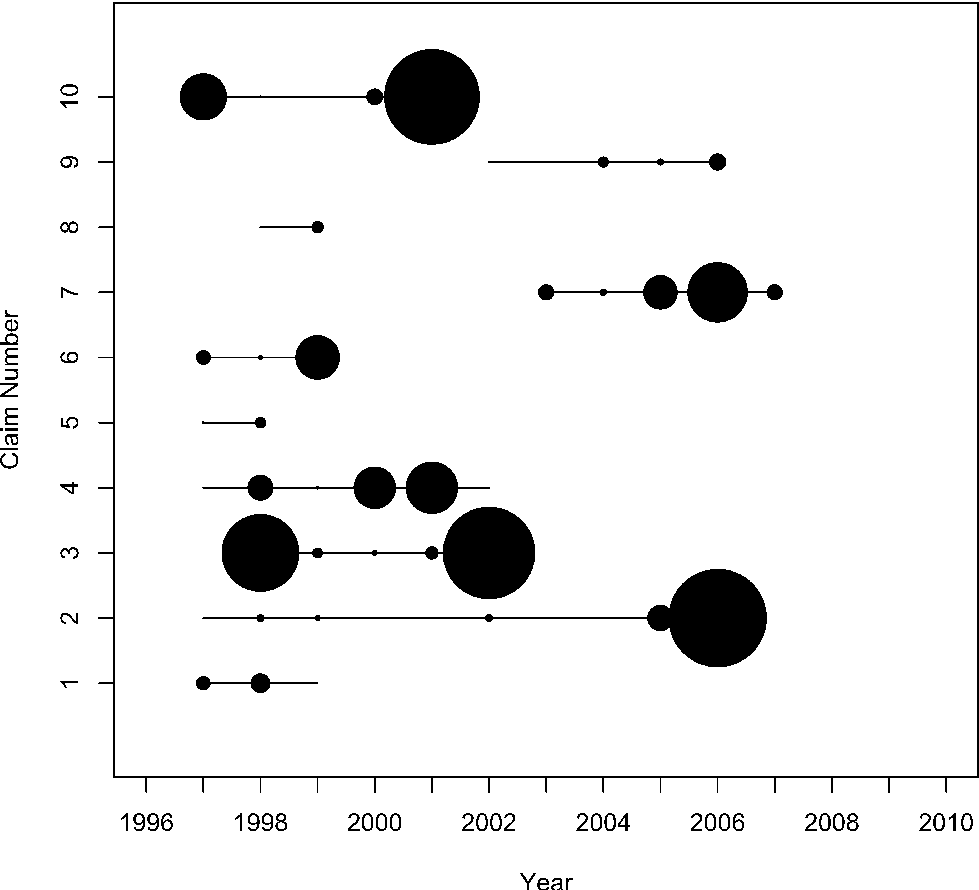
\includegraphics[height=0.45\textwidth, width=0.45\textwidth]{images/E1a}
  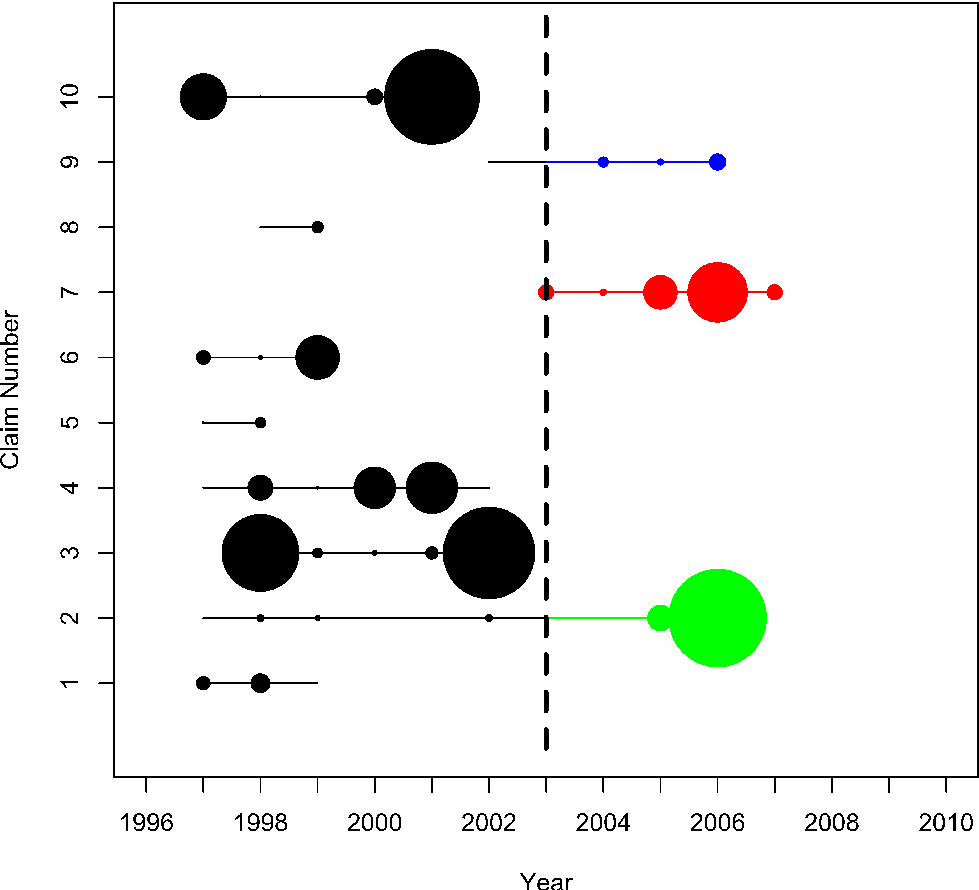
\includegraphics[height=0.45\textwidth, width=0.45\textwidth]{images/E2a}
  \caption{Exemples de classification des sinistres. Le graphique de
    gauche présente l'évolution de $10$ sinistres, les tailles des
    points étant proportionnelles aux montants payés. En supposant que
    l'évaluation a lieu le 1 janvier 2003, le graphique de droite
    présente la classification des sinistres: les sinistres
    1,3,4,5,6,8 et 10 sont S, le sinistre 2 est RBNS, le sinistre 7
    est IBNR et le sinistre 9 est RBNP.}
  \label{fig:presentation:E1E2}
\end{figure}

En plus du développement que l'on vient de décrire, une compagnie
d'assurance détient généralement une certaine expérience via ses
experts. Cette expérience se traduira par des prédictions du montant
total d'un sinistre réalisées à différents moments entre la date de
déclaration et la date de fermeture d'un dossier. Ce processus est
illustré à la \autoref{fig:presentation:evolRES}. Il est à noter qu'un
changement dans le montant prédit de réserve n'accompagne pas
nécessairement un paiement.

Il faut alors chercher à construire un modèle permettant de
représenter l'évolution des sinistres et à estimer les paramètres de
ce modèle à partir de l'information disponible.

\begin{figure}
  \centering
  \setlength{\unitlength}{5mm}
  \small
  \begin{picture}(22,10)
    \put(1,5){\vector(1,0){21}}
    \put(1,3){\vector(1,0){21}}
    \put(2,9){\vector(0,-1){3}}
    \put(4,7){\vector(0,-1){1}}
    \put(9,9){\vector(0,-1){3}}
    \put(10,9){\vector(0,-1){3}}
    \put(11,9){\vector(0,-1){3}}
    \put(20,9){\vector(0,-1){3}}
    \put(2,4.75){\line(0,1){0.5}}
    \put(4,4.75){\line(0,1){0.5}}
    \put(9,4.75){\line(0,1){0.5}}
    \put(10,4.75){\line(0,1){0.5}}
    \put(11,4.75){\line(0,1){0.5}}
    \put(20,4.75){\line(0,1){0.5}}
    % \put(2,2.75){\line(0,1){0.5}}
    \put(4,2.75){\line(0,1){0.5}}
    \put(9,2.75){\line(0,1){0.5}}
    \put(10,2.75){\line(0,1){0.5}}
    % \put(11,2.75){\line(0,1){0.5}}
    \put(20,2.75){\line(0,1){0.5}}
    \put(15,2.75){\line(0,1){0.5}}

    \put(2,4){$t_1$} \put(4,4){$t_2$}
    \put(9,4){$t_3$} \put(10,4){$t_4$}
    \put(11,4){$t_5$}
    \put(15,4){$t_{5.5}$}
    \put(20,4){$t_6$}
    \put(0.5,10){Survenance}
    \put(2.5,8){Déclaration}
    \put(8,10){Paiements}
    \put(19,10){Fermeture}

    \put(3,0){Réserve}
    \put(3,-1){initiale}
    \put(11,0){Ajustements}
    \put(19,0){Fermeture}
    \put(4,1){\vector(0,1){1}}
    \put(9,1){\vector(0,1){1}}
    \put(10,1){\vector(0,1){1}}
    \put(15,1){\vector(0,1){1}}
    \put(20,1){\vector(0,1){1}}

    % \put(2,-1.5){\textcolor{rougeG}{\line(1,0){2}}}
    % \put(2,-1.75){\textcolor{rougeG}{\line(0,1){0.5}}}
    % \put(4,-1.75){\textcolor{rougeG}{\line(0,1){0.5}}}
    % \put(2,-2.75){\textcolor{rougeG}{IBNR}}

    % \put(4,-2.5){\textcolor{bleuG}{\line(1,0){5}}}
    % \put(4,-2.75){\textcolor{bleuG}{\line(0,1){0.5}}}
    % \put(9,-2.75){\textcolor{bleuG}{\line(0,1){0.5}}}
    % \put(6,-3.75){\textcolor{bleuG}{RBNP}}
    % \put(9,-1.5){\textcolor{green}{\line(1,0){11}}}
    % \put(9,-1.75){\textcolor{green}{\line(0,1){0.5}}}
    % \put(20,-1.75){\textcolor{green}{\line(0,1){0.5}}}
    % \put(14,-2.75){\textcolor{green}{RBNS}}

    % \put(3, 1){\circle*{.5}}
  \end{picture}
  \caption{Évaluations des experts}
  \label{fig:presentation:evolRES}
\end{figure}


\section{Approches collectives et individuelles}
\label{sec:presentation:approches}

L'estimation des paramètres d'un modèle décrivant en détail le
développement individuel des sinistres (voir la
\autoref{fig:presentation:evolIN}) demande une base de données
détaillée (dates exactes, montant de chacun des paiements, etc.) et
fiable, de même que des moyens calculatoires (informatiques)
importants. De telles ressources n'étant disponibles que depuis peu
(fin des années 90 environ), plusieurs modèles ont été développés pour
représenter la \emph{dynamique collective} des sinistres\footnote{%
  De nombreuses autres raisons peuvent motiver l'utilisation
  d'approches collectives: la simplicité et la robustesse des modèles
  collectifs, le risque de sur-paramétrisation des approches
  individuelles, etc. Une comparaison des approches collectives et
  individuelles est réalisée dans \cite{Jin2014}.}. %

\subsection{Approches collectives}
\label{sec:presentation:approches:collectives}

Les modèles collectifs pour les réserves ont été étudiés
principalement depuis le début des années 80. Parmi ces modèles, le
modèle \emph{Chain--Ladder} (ou modèle de Mack dans sa version
stochastique, voir \cite{Mack93}) occupe une position particulière
étant à la base de la plupart des modèles utilisés en pratique. Ce
modèle (de même que ses nombreuses extensions et variantes) est
construit à partir d'une base de données résumées par période
(typiquement une année) de survenance et par période de développement
en un tableau nommé \emph{triangle de développement} (voir
\autoref{sec:presentation:triangles}). Ces modèles seront étudiés dans
les deux prochains chapitres.

À partir de cette même structure, ou à partir d'une version
\emph{incrémentale} de cette dernière, plusieurs modèles paramétriques
ont également été proposés (voir \citet{Hertig}, \citet{RV98},
\citet{EV2005} et \citet{Taylorbook}). Ces modèles s'inscrivent plus
ou moins directement dans la théorie des modèles linéaires généralisés
(\emph{Generalized Linear Models}) et des modèles linéaires
généralisés mixtes (\emph{Generalized Linear Mixed Models}) et seront
brièvement introduits au Chapitre 9. Un lecteur intéressé par un
historique plus complet des modèles collectifs est invité à consulter
\citet{WuthrichBook} et \citet{Engl02}.

\subsection{Approches individuelles}
\label{sec:presentation:approches:individuelles}

Très récemment, des modèles individuels ont commencé à faire leur
apparition dans la littérature. Les articles \citet{Arjas} et
\citet{Norberg, Norberg99} ont proposé une structure stochastique
individuelle en temps continu pour les sinistres et l'évaluation des
réserves. À partir de cette base, quelques modèles ont été développés,
par exemple \citet{Haastrup}, \citet{Lars07}, \citet{Zhao09},
\citet{ZhaoIME2} et \citet{AntonioPlat}. À l'exception notable de ce
dernier article, aucune mise en pratique réaliste de ces modèles n'a
été réalisée. Dans une autre voie, des modèles individuels basés sur
la structure \emph{chain--ladder} ont été proposés (voir
\citet{PigAntDen2013} et \citet{PigAntDen2014}). Enfin, quelques
modèles non-paramétriques ont également été proposés (voir
\citet{Drieskens} et \citet{Rosenlund} par exemple). Les approches
individuelles ne seront pas traitées dans le cadre de ce cours.

\begin{exemple}
  On considère un cas d'assurance responsabilité civile automobile
  (blessure corporelle):
  \begin{itemize}
  \item le 15 novembre 2004, un assuré frappe un piéton avec sa
    voiture;
  \item le 10 janvier 2005, le piéton commence à ressentir de violents
    maux de dos et de tête, conséquences de l'accident. Une poursuite
    est engagée contre le conducteur par le piéton;
  \item le 22 janvier 2005, l'assuré contacte son assureur pour
    l'avertir de la réclamation et le service d'indemnisation de la
    compagnie d'assurance évalue automatiquement la réclamation à
    \nombre{20 000}~\$;
  \item le 1er mars 2005, des spécialistes de la compagnie d'assurance
    évalue la réclamation à \nombre{200 000}~\$;
  \item le 30 mars 2005, le piéton refuse l'offre de \nombre{180
      000}~\$ de la compagnie d'assurance et va en cour;
  \item le 30 juin 2005, la compagnie d'assurance paie \nombre{15
      000}~\$ de frais légaux pour les services d'avocat (pour cette
    cause);
  \item le 30 mai 2006, la compagnie d'assurance paie \nombre{30
      000}~\$ de frais légaux pour les services d'avocat (pour cette
    cause);
  \item Le 6 octobre 2007, la décision de la cour est une indemnité de
    \nombre{250000}~\$.
  \end{itemize}
  Illustrer par une ligne du temps la vie du sinistre.

  Dessin à faire...

  \textbf{Remarques: }
  \begin{itemize}
  \item le 31 décembre 2004, la compagnie se devait d'inscrire une
    réserve pour l'accident du 15 novembre;
  \item aucune réclamation n'avait pourtant été soumise;
  \item ce genre de provisions s'appelle IBNR (\emph{Incurred But Not
      Reported});
  \item des paiements ont lieu tout au long de la vie de la
    réclamation;
  \item le 31 décembre 2005 et 2006, la compagnie se devait d'inscrire
    pour l'année d'accident 2004, une réserve pour ce sinistre;
  \item le 31 décembre 2007, malgré qu'il semble que le sinistre soit
    clos, il existe peut-être une possibilité de réouverture du
    dossier...
  \end{itemize}
  \qed
\end{exemple}

Lors de l'estimation des réserves, certaines hypothèses sont utilisées:
\begin{itemize}
\item les techniques d'évaluation des réserves seront utilisées avec
  des dollars constants; et
\item aucune actualisation des montants n'est considérée.
\end{itemize}

Pendant longtemps, l'actualisation des réserves a été illégale dans
l'évaluation du passif des polices et ce, même si l'effet du facteur
d'escompte n'est pas négligeable sur des branches d'assurance très
longues.

%\begin{definition}[Réserve individuelle de sinistre]
%Il s'agit de l'estimation, réalisée par les
%spécialistes de la compagnie d'assurance, du montant total qu'il reste à payer pour u%n sinistre. Cette estimation est
%réalisée au moment de l'évaluation (à l'instant présent).
%\end{definition}

%\begin{definition}[Sinistres survenus mais non-rapportés (\textit{IBNR})]
%Il s'agit de sinistres (ou de montants de sinistres) qui sont survenus
%mais dont l'assureur ne connaît pas encore l'existence.
%\end{definition}

%Les pertes totales, ou encore l'encouru total, pour un
%assureur correspond à tout ce qu'il a payé et tout ce qu'il lui reste
%à payer (réserve).  De manière plus rigoureuse, on peut
%définir les éléments d'une réserve.

%\begin{definition}
%Une réserve est composée des éléments suivants:
%\begin{itemize}
%\item les réserves individuelles;
%\item les ajustements à venir des réserves individuelles;
%\item les sinistres survenus mais non-rapportés (IBNR);
%\item les réclamations fermées qui peuvent rouvrir; et
%\item les sinistres rapportés mais non-enregistrés.
%\end{itemize}
%\end{definition}

La dynamique de la vie des sinistres dépend beaucoup de la ligne
d'affaires. Pour un type de risque particulier, les sinistres sont
constatés (avec plus ou moins de retard), puis ensuite payés, encore
avec plus ou moins de retard.

Pour fin d'illustration, si un accident a lieu durant l'année $T$, le
\autoref{tab:presentation:plo} donne une idée des cadences de
règlement pour différentes branches d'assurance.

\begin{table}
  \centering
  \caption{Cadences de règlement pour différentes branches
    d'assurance}
  \label{tab:presentation:plo}
  \begin{tabular}{llllll}
    \toprule
    Règlements à la fin de l'année  & $T$ & $T+1$ & $T+2$ & $T+3$ & $T+4$\\
    \midrule
    Multirisque habitation & $55~\%$ & $90~\%$ & $94~\%$ & $95~\%$ & $96~\%$ \\
    Automobile & $55~\%$ & $79~\%$ & $84~\%$ & $89~\%$ & $90~\%$ \\
    \textit{dont corporel} & $13~\%$ & $38~\%$ & $50~\%$ & $65~\%$ & $72~\%$ \\
    Responsabilité civile & $10~\%$ & $25~\%$ & $35~\%$ & $40~\%$ & $45~\%$ \\
    \bottomrule
  \end{tabular}
\end{table}

Le but principal des deux chapitres à venir est de développer des
techniques afin d'estimer le plus précisément possible le montant des
réserves pour chacun des bilans financiers de l'assureur, c'est-à-dire
à la fin des années $T$, $T+1$, etc. Ainsi, on peut établir l'équation
suivante:
\begin{align*}
  \text{Réserve estimée}
  &= \text{Pertes ultimes estimées} - \text{montants payés}\\
  % &= (\text{montants payés} + \text{Réserves individuelles} + \text{IBNR} + \ldots)  - %\text{montants payés}\\
  &= \text{Réserves RBNS} + \text{Réserves IBNR} \\
  &\phantom{=} + \text{Réclamations fermées qui peuvent rouvrir}.
\end{align*}


\section{Techniques intuitives}
\label{sec:presentation:techniques}

Dans certaines situations où les paiements futurs sont très stables et
très prévisibles, il est possible d'utiliser des méthodes simples pour
l'estimation des réserves.

\begin{description}
\item[Méthode des réserves enregistrées] L'idée de la méthode est
  d'utiliser le total des estimations faites par les experts de la
  compagnie (les réserves enregistrées) et d'ajouter un pourcentage
  arbitraire afin d'inclure l'incertitude quant à l'évolution possible
  des coûts futurs. Le problème majeur de cette méthode est d'estimer
  correctement ce pourcentage.

\item[Méthode des rapports sinistres/primes espérés] L'idée de la
  méthode est d'utiliser le rapport sinistres/primes prédit (attendu)
  de la branche d'affaire et les montants payés à ce jour de
  réclamations afin d'estimer la réserve. Ainsi, pour une année $i$
  fixée, on a
  \begin{align*}
    \text{Pertes ultimes estimées}_i
    &= \left(\text{Rapport sinistres/primes espéré}\right)_i \times \text{Primes acquises}_i\\
    \text{Réserve estimée}_i
    &= \text{Pertes ultimes estimées}_i - \text{Montants payés}_i
  \end{align*}
  En sommant toutes les années de couverture, on obtient une
  estimation de la réserve:
  \begin{align*}
    \text{Réserve estimée totale} &= \sum_i \text{Réserve estimée}_i.
  \end{align*}
\end{description}

\begin{exemple}
  On considère les primes acquises et les montants totaux payés à la
  fin de 2005, présentés dans le tableau ci-dessous, pour les années
  2000 à 2005:
  \begin{center}
    \begin{tabular}{|c | c c|}\hline
      Année & Primes acquises & Montants payés \\ \hline
      2000 & $\nombre{100000}$ & $\nombre{58000}$\\
      2001 & $\nombre{105000}$ & $\nombre{50000}$\\
      2002 & $\nombre{110000}$ & $\nombre{45000}$\\
      2003 & $\nombre{112500}$ & $\nombre{40000}$\\
      2004 & $\nombre{120000}$ & $\nombre{25000}$\\
      2005 & $\nombre{115000}$ & $\nombre{12000}$ \\ \hline
    \end{tabular}
  \end{center}

  Estimer la réserve totale pour les années 2000 à 2005 si on prévoit
  un rapport sinistres/primes de $60~\%$ pour toutes les années.

  \begin{align*}
    \text{Primes acquises}_{total}
    &= \nombre{662500}\\
    \text{Pertes ultimes estimées}_{total}
    &= \left(\text{Rapport sinistres/primes espéré}\right)_{total} \times \text{Primes acquises}_{total}\\
    &= 0,60 \times \nombre{662500} = \nombre{397500}\\
    \text{Réserve estimée}_{total}
    &= \text{Pertes ultimes estimées}_{total} - \text{montants payés}_{total}\\
    &=  \nombre{397500} - \nombre{230000} = \nombre{167500}.
  \end{align*}
  Cette méthode souffre du problème qu'il est plus que probable que
  les pertes soient différentes de celles prévues (catastrophe,
  etc.). %
  \qed
\end{exemple}


\section{Triangles de développement}
\label{sec:presentation:triangles}

Afin d'étudier l'évolution des coûts au cours du temps et de pouvoir
estimer les réserves d'une compagnie d'assurance, on considère
généralement les données sous la forme d'un triangle de développement.
Ce dernier reflète la dynamique collective des sinistres.

La notation usuelle est la suivante:
\begin{itemize}
\item $i$ correspond à l'indice des années de survenance
  $i = 1, \ldots, I$;
\item $j$ correspond à l'indice des années de développement
  $j = 1, \ldots, J$;
\item $Y_{i,j}$ correspond au montant des sinistres survenus l'année
  $i$ et payés l'année $i + j$ (ou après $j$ années de développement).
  Pour cette variable, on parle aussi d'incréments; et
\item $C_{i,j}$ correspond aux paiements agrégés des sinistres
  survenus l'année $i$, en $j$ années de développement, i.e.
  $C_{i,j} = Y_{i,1} + Y_{i,2} + \ldots + Y_{i,j}$. Pour cette
  variable, on parle aussi de montants cumulés.
\end{itemize}

La sinistralité d'une branche peut ainsi être représentée par
\begin{center}
  \begin{tabular}{*{8}{c}}
    \toprule
    Année & \multicolumn{7}{c}{Développement (âge)} \\
    accident & $1$ & $2$ & $\cdots$ & $j$ & $\cdots$ & $J - 1$ & $J$ \\
    \midrule
    $1$ & $C_{1, 1}$ & $C_{1, 2}$ & $\cdots$ & $C_{1, j}$ & $\cdots$ & $C_{1, J-1}$ & $C_{1, J}$ \\
    $2$ & $C_{2, 1}$ & $C_{2, 2}$ & $\cdots$ & $C_{2, j}$ & $\cdots$ & $C_{2, J-1}$ \\
    $\vdots$ \\
    $i$ & $C_{i, 1}$ & $C_{i, 2}$ & $\cdots$ & $C_{i, j}$ \\
    $\vdots$ \\
    $I - 1$ & $C_{I-1, 1}$ & $C_{I-1, 2}$ \\
    $I$ & $C_{I, 1}$ \\
    \bottomrule
  \end{tabular}
\end{center}
ou
\begin{center}
  \begin{tabular}{*{8}{c}}
    \toprule
    Année & \multicolumn{7}{c}{Développement (âge)} \\
    accident & $1$ & $2$ & $\cdots$ & $j$ & $\cdots$ & $J - 1$ & $J$ \\
    \midrule
    $1$ & $Y_{1, 1}$ & $Y_{1, 2}$ & $\cdots$ & $Y_{1, j}$ & $\cdots$ & $Y_{1, J-1}$ & $Y_{1, J}$ \\
    $2$ & $Y_{2, 1}$ & $Y_{2, 2}$ & $\cdots$ & $Y_{2, j}$ & $\cdots$ & $Y_{2, J-1}$ \\
    $\vdots$ \\
    $i$ & $Y_{i, 1}$ & $Y_{i, 2}$ & $\cdots$ & $Y_{i, j}$ \\
    $\vdots$ \\
    $I - 1$ & $Y_{I-1, 1}$ & $Y_{I-1, 2}$ \\
    $I$ & $Y_{I, 1}$ \\
    \bottomrule
  \end{tabular}
\end{center}

La lecture des triangles de développement peut se faire selon divers
angles:
\begin{itemize}
\item la lecture par \textbf{colonne} correspond à l'année de
  développement $j$, et reflète l'évolution de la vie des sinistres;
\item la lecture par \textbf{ligne} correspond à l'année de survenance
  $i$, et reflète les changements de souscriptions, de taille du
  portefeuille, etc.; et
\item la lecture par \textbf{diagonale} correspond à l'année de
  calendrier.
\end{itemize}

\begin{exemple}
  On considère le triangle de paiements suivant (pour aider à la
  notation, on suppose que la première année est l'année 1997):
  \begin{center}
    \begin{tabular}{*{6}{c}}
      \toprule
      Année & \multicolumn{5}{c}{Développement (âge)} \\
      accident& 12 mois & 24 mois & 36 mois & 48 mois & 60 mois \\
      \midrule
      1997 & $\nombre{26312}$ & $\nombre{31467}$ & $\nombre{24672}$ & $\nombre{13055}$ & $\nombre{6158}$ \\
      1998 & $\nombre{30470}$ & $\nombre{35012}$ & $\nombre{25491}$ & $\nombre{12589}$ \\
      1999 & $\nombre{49756}$ & $\nombre{51831}$ & $\nombre{35267}$ \\
      2000 & $\nombre{50420}$ & $\nombre{52315}$ \\
      2001 & $\nombre{56762}$ \\
      \bottomrule
    \end{tabular}
  \end{center}
  Calculer les éléments suivants:

  \begin{itemize}
  \item les montants payés en 1999 pour les sinistres survenus pendant
    l'année 1999;
  \item les montants payés en 1999 pour les sinistres survenus pendant
    l'année 1997; et
  \item le montant total des sinistres payés pour l'année de
    survenance 1998 observé à la fin de l'année 2000.
  \end{itemize}

  On obtient
  \begin{itemize}
  \item En 1999, $\nombre{49756}$~\$ ont été payés pour les sinistres
    survenus à l'année 1999;
  \item $\nombre{24672}$~\$ ont été payés pour des sinistres survenus
    en 1997; et
  \item le montant total des sinistres payés pour l'année de
    survenance 1998 était, à la fin de 2000, de
    $\nombre{90973} = \nombre{30470} + \nombre{35012} +
    \nombre{25491}$.
  \end{itemize}
  \qed
\end{exemple}

Puisque l'idée du provisionnement est de \textbf{prévoir le montant
  final des sinistres} afin de provisionner pour les paiements
non-effectués, sous l'hypothèse que tous les sinistres seront réglés
après $J$ années, on cherche à compléter le tableau en remplissant le
triangle inférieur droit
\begin{center}
  \begin{tabular}{*{8}{c}}
    \toprule
    Année & \multicolumn{7}{c}{Développement (âge)} \\
    accident & $1$ & $2$ & $\cdots$ & $j$ & $\cdots$ & $J - 1$ & $J$ \\
    \midrule
    $1$ & $C_{1, 1}$ & $C_{1, 2}$ & $\cdots$ & $C_{1, j}$ & $\cdots$ & $C_{1, J-1}$ & $C_{1, J}$ \\
    $2$ & $C_{2, 1}$ & $C_{2, 2}$ & $\cdots$ & $C_{2, j}$ & $\cdots$ & $C_{2, J-1}$ & $\hat{C}_{1, J}$ \\
    $\vdots$ \\
    $i$ & $C_{i, 1}$ & $C_{i, 2}$ & $\cdots$ & $C_{i, j}$ & $\cdots$ & $\hat{C}_{i, J-1}$ & $\hat{C}_{1, J}$ \\
    $\vdots$ \\
    $I - 1$ & $C_{I-1, 1}$ & $C_{I-1, 2}$  & $\cdots$ & $\hat{C}_{i, j}$ & $\cdots$ & $\hat{C}_{i, J-1}$ & $\hat{C}_{1, J}$ \\
    $I$ & $C_{I, 1}$ & $\hat{C}_{I-1, 2}$  & $\cdots$ & $\hat{C}_{i, j}$ & $\cdots$ & $\hat{C}_{i, J-1}$ & $\hat{C}_{1, J}$ \\
    \bottomrule
  \end{tabular}
\end{center}
ou
\begin{center}
  \begin{tabular}{*{8}{c}}
    \toprule
    Année & \multicolumn{7}{c}{Développement (âge)} \\
    accident & $1$ & $2$ & $\cdots$ & $j$ & $\cdots$ & $J - 1$ & $J$ \\
    \midrule
    $1$ & $Y_{1, 1}$ & $Y_{1, 2}$ & $\cdots$ & $Y_{1, j}$ & $\cdots$ & $Y_{1, J-1}$ & $Y_{1, J}$ \\
    $2$ & $Y_{2, 1}$ & $Y_{2, 2}$ & $\cdots$ & $Y_{2, j}$ & $\cdots$ & $Y_{2, J-1}$ & $\hat{C}_{1, J}$ \\
    $\vdots$ \\
    $i$ & $Y_{i, 1}$ & $Y_{i, 2}$ & $\cdots$ & $Y_{i, j}$ & $\cdots$ & $\hat{C}_{i, J-1}$ & $\hat{C}_{1, J}$ \\
    $\vdots$ \\
    $I - 1$ & $Y_{I-1, 1}$ & $Y_{I-1, 2}$  & $\cdots$ & $\hat{C}_{i, j}$ & $\cdots$ & $\hat{C}_{i, J-1}$ & $\hat{C}_{1, J}$ \\
    $I$ & $Y_{I, 1}$ & $\hat{C}_{I-1, 2}$  & $\cdots$ & $\hat{C}_{i, j}$ & $\cdots$ & $\hat{C}_{i, J-1}$ & $\hat{C}_{1, J}$ \\
    \bottomrule
  \end{tabular}
\end{center}

Ayant estimé ces paiements futurs, le montant des provisions pour
l'année de survenance $i$ est alors donné par
\begin{align*}
  \hat{R}_i &= \hat{C}_{i,n} - C_{i, n+1-i} =
                  \hat{Y}_{i,n+2-i} + \hat{Y}_{i,n+3-i} + \dots +
                  \hat{Y}_{i,n}
\end{align*}
et le montant total des réserves est donné par
\begin{align*}
R &= \sum_{i=1}^n \hat{R}_i = \sum_{i=1}^n \hat{C}_{i,n} -
C_{i, n+1-i} = \sum_{(i,j) \in \Delta_n } \hat{Y}_{i,j},
\end{align*}
où $\Delta_I$ désigne l'ensemble
$\{(i, j), i + j \ge I + 2, i \le I \text{ et } j \le J \}$.

Les modèles basés sur les triangles de développement supposent souvent
que tous les sinistres sont réglés après $J$ années. Afin d'assouplir
cette condition, il est aussi possible de considérer des ajustement
pour tenir compte des futures évolutions.


\section{Exercices}
\label{sec:presentation:exercices}

\Opensolutionfile{reponses}[reponses-presentation]
\Opensolutionfile{solutions}[solutions-presentation]

\begin{Filesave}{reponses}
\bigskip
\section*{Réponses}

\end{Filesave}

\begin{Filesave}{solutions}
\section*{Chapitre \ref*{chap:presentation}}
\addcontentsline{toc}{section}{Chapitre \protect\ref*{chap:presentation}}

\end{Filesave}

\begin{exercice}
 Le \autoref{tab:presentation:loss12} présente les différents paiements
 réalisés par l'assureur YTR.
  \begin{table}[!h]
    \centering
    \caption{Paiements réalisés par l'assureur YTR}
    \label{tab:presentation:loss12}
    \begin{tabular}{cccc}
      \toprule
      Date paiement & Numéro assuré & Date survenance & Montant\\
      \midrule
      04/2000 & 456 & 03/2000 & $200$\\
      09/2000 & 476 & 08/2000 & $225$\\
      02/2001 & 456 & 03/2000 & $40$\\
      10/2001 & 476 & 08/2000 & $57$\\
      01/2002 & 456 & 03/2000 & $90$\\
      04/2003 & 476 & 08/2000 & $102$\\
      02/2004 & 476 & 08/2000 & $16$\\
      10/2001 & 287 & 10/2001 & $532$\\
      12/2002 & 287 & 10/2001 & $125$\\
      02/2003 & 937 & 03/2001 & $57$\\
      01/2004 & 287 & 10/2001 & $18$\\
      05/2002 & 456 & 03/2002 & $717$\\
      08/2003 & 456 & 03/2002 & $13$\\
      04/2004 & 456 & 03/2002 & $72$\\
      07/2003 & 101 & 07/2003 & $440$\\
      01/2004 & 867 & 03/2003 & $120$\\
      04/2004 & 200 & 02/2004 & $400$\\
      10/2004 & 956 & 08/2004 & $220$\\
      \bottomrule
    \end{tabular}
  \end{table}
  \begin{enumerate}
  \item Construire les triangles des paiements cumulés.
  \item Quel est le nombre de périodes nécessaires pour observer le
    développement complet des paiements?
  \end{enumerate}
  \begin{rep}
    \begin{enumerate}
      \stepcounter{enumii}
    \item $5$
    \end{enumerate}
  \end{rep}
  \begin{sol}
    \begin{enumerate}
    \item Le triangle des paiements cumulés est présenté dans le
      \autoref{tab:presentation:tri1}. Pour la case $(i, j)$, il suffit de
      sommer les montants des paiements pour les sinistres survenus
      pendant l'année~$i$ et payés pendant la $j\ieme$~période après
      la survenance.
      \begin{table}[!h]
        \centering
        \caption{Paiements réalisés par l'assureur YTR}
        \label{tab:presentation:tri1}
        \begin{tabular}{cccccc}
          \toprule
          & $1$ & $2$ & $3$ & $4$ & $5$\\
          \midrule
          2000 & $425$ & $522$ & $612$ & $714$ & $730$\\
          2001 & $532$ & $657$ & $714$ & $732$ & -\\
          2002 & $717$ & $730$ & $802$ & - & -\\
          2003 & $440$ & $560$ & - & - & -\\
          2004 & $620$ & - & - & - & -\\
          \bottomrule
        \end{tabular}
      \end{table}
    \item Selon les données enregistrées par la compagnie, il est
      raisonnable de supposer que les paiements sont pratiquement
      complets après $5$~périodes de développement. Idéalement, le
      fait de pouvoir consulter une base de données semblables plus
      mature permettrait de confirmer ou d'infirmer cette hypothèse.
      Enfin, connaître le type de portefeuille (assurance automobile -
      dommage matériel, assurance automobile - dommage corporel,
      assurance responsabilité professionnelle, etc.) permettrait
      également d'avoir une idée du nombre de périodes de
      développement nécessaires.
    \end{enumerate}
  \end{sol}
\end{exercice}

\begin{exercice}
  On considère les primes acquises et les montants totaux payés
  suivants, à la fin de 2005, pour les années 2000 à 2005.
  \begin{center}
    \begin{tabular}{|c | c c c |}\hline
      Année & Primes acquises & Montants payés & Rapport sinistres/primes espéré\\ \hline
      2000 & $\numprint{200000}$ & $\numprint{158000}$ & $85~\%$\\
      2001 & $\numprint{205000}$ & $\numprint{150000}$ & $87,5~\%$\\
      2002 & $\numprint{210000}$ & $\numprint{145000}$ & $85~\%$\\
      2003 & $\numprint{212500}$ & $\numprint{140000}$ & $78~\%$\\
      2004 & $\numprint{220000}$ & $\numprint{125000}$ & $80~\%$\\
      2005 & $\numprint{215000}$ & $\numprint{112000}$ & $75~\%$ \\ \hline
    \end{tabular}
  \end{center}
  En utilisant la méthode des rapports sinistres/primes espérés,
  estimer la réserve totale pour les années 2000 à 2005.
  \begin{rep}
    $\numprint{200875}$
  \end{rep}
  \begin{sol}
    On a
    \begin{align*}
      \text{Pertes ultimes estimées}_{2000} &= \text{Rapport
                                              sinistres/primes espéré}_{2000} \times \text{Primes
                                              acquises}_{2000}\\
                                            &= (0,85)(\numprint{200000}) = \numprint{170000}\\
      \text{Pertes ultimes estimées}_{2001} &= \numprint{179375}\\
      \text{Pertes ultimes estimées}_{2002} &= \numprint{178500}\\
      \text{Pertes ultimes estimées}_{2003} &= \numprint{165750}\\
      \text{Pertes ultimes estimées}_{2004} &= \numprint{176000}\\
      \text{Pertes ultimes estimées}_{2005} &= \numprint{161250}\\
      \text{Pertes ultimes estimées}_{Total} &= \numprint{1030875}\\
      \text{Réserve estimée}_{total} &= \text{Pertes ultimes estimées}_{total} - \text{montants payés}_{total}\\
                                            &=  \numprint{1030875} - \numprint{830000} = \numprint{200875}.
    \end{align*}
  \end{sol}
\end{exercice}

\begin{exercice}
  On considère les primes acquises et les réserves individuelles de
  chaque sinistre, à la fin de 2005, pour les années 2000 à 2005
  \begin{center}
    \begin{tabular}{|c | c c|}\hline
      Année & Primes acquises & Somme des réserves individuelles \\ \hline
      2000 & $\numprint{100000}$ & $\numprint{58000}$\\
      2001 & $\numprint{105000}$ & $\numprint{50000}$\\
      2002 & $\numprint{110000}$ & $\numprint{45000}$\\
      2003 & $\numprint{112500}$ & $\numprint{40000}$\\
      2004 & $\numprint{120000}$ & $\numprint{25000}$\\
      2005 & $\numprint{115000}$ & $\numprint{12000}$ \\ \hline
    \end{tabular}
  \end{center}
  En utilisant la méthode des réserves enregistrées, estimer la
  réserve totale pour les années 2000 à 2005 si on utilise un facteur
  de $5~\%$.
  \begin{rep}
    $\numprint{241500}$
  \end{rep}
  \begin{sol}
    La somme des réserves individuelles est $\numprint{230000}$.
    Ainsi, la réserve totale est
    $(\numprint{230000})(1,05) = \numprint{241500}$.
  \end{sol}
\end{exercice}

\begin{exercice}
  L'actuaire de la compagnie \textbf{GFR} possède les informations
  suivantes sur les montants payés cumulatifs, en fonction des années
  de développement et de l'année de survenance du sinistre:
  \begin{center}
    \begin{tabular}{|l|l l l l l l l|}\hline
      Année & $1$ & $2$ & $3$ & $4$ & $5$ & $6$ & $7$\\ \hline
      1993 & $\numprint{1780}$ & $\numprint{2673}$ & $\numprint{2874}$ & $\numprint{3094}$ & $\numprint{3157}$ & $\numprint{3166}$ & $\numprint{3166}$ \\
      1994 & $\numprint{3226}$ & $\numprint{4219}$ & $\numprint{4532}$ & $\numprint{4881}$ & $\numprint{5144}$ & $\numprint{5199}$ & \\
      1995 & $\numprint{3652}$ & $\numprint{4989}$ & $\numprint{5762}$ & $\numprint{6436}$ & $\numprint{6720}$ & & \\
      1996 & $\numprint{2723}$ & $\numprint{4301}$ & $\numprint{5526}$ & $\numprint{6231}$ & & & \\
      1997 & $\numprint{2923}$ & $\numprint{4666}$ & $\numprint{5349}$ & & & & \\
      1998 & $\numprint{2990}$ & $\numprint{5417}$ & & & & & \\
      1999 & $\numprint{3917}$ & & & & & &\\ \hline
    \end{tabular}
  \end{center}

  \begin{enumerate}
  \item Combien de dollars ont été payés pour les sinistres survenus
    en 1993 ?
  \item En 1997, combien de dollars ont été payés pour les sinistres
    survenus en 1995 ?
  \item Quel est le montant total de sinistres payés pour l'année de
    survenance 1998 ?
  \item Combien de dollars ont été payés en indemnités pendant l'année
    1999 ?
  \item Combien de dollars ont été payés en indemnités pendant l'année
    1994 ?
  \end{enumerate}

  \begin{rep}
    \begin{enumerate}
    \item $\numprint{3166}$
    \item $\numprint{773}$
    \item $\numprint{5417}$
    \item $\numprint{8071}$
    \item $\numprint{4119}$
    \end{enumerate}
  \end{rep}
  \begin{sol}
    \begin{enumerate}
    \item Le dernier montant cumulatif disponible pour l'année de
      survenance 1993 est $\numprint{3166}$~\$.
    \item On calcule $\numprint{5762} - \numprint{4989} = 773$.
    \item Le dernier montant cumulatif disponible pour l'année de
      survenance 1998 est $\numprint{5417}$.
    \item On calcule $\numprint{3917} +
      (\numprint{5417}-\numprint{2990}) + (\numprint{5349} -
      \numprint{4666}) + (\numprint{6231} - \numprint{5526}) +
      (\numprint{6720}-\numprint{6436}) + (\numprint{5199} -
      \numprint{5144}) + 0 = \numprint{8071}$.
    \item On calcule $\numprint{3226} +
      (\numprint{2673}-\numprint{1780}) = \numprint{4119}$.
    \end{enumerate}
  \end{sol}
\end{exercice}

\Closesolutionfile{solutions}
\Closesolutionfile{reponses}

%%% Local Variables:
%%% mode: latex
%%% TeX-master: "provisionnement-assurance-iard"
%%% TeX-engine: xetex
%%% coding: utf-8
%%% End:
